\chapter{State of the art}
\label{ch:background}

\section{Ant Colony Optimization}

Ant Colony Optimization(ACO) have been around for quite some time, and there are sevral different applications this algoritm can be used for, for example routing, scheduling, subset and machine learning[1]. The offical website to ACO is www.aco-metaheuristic.org. There are several different ACO systems that have been developed, two of the most successful are MAX-MIN Ant system and Ant Colony system.

In the orignial Ant system, each iteration runs m ants through the different paths/graph, and creates a solution. When all the m ants have finished, the update to pheromones happens to the solution the ants have found. Then the algorithm starts the next iteration with the next m ants.

MAX-MIN Ant system is an improvement to the original in the way that only the best solution is updated or best so far.

Ant Colony system uses “local pheromones” and “offline pheromones” in finding the best solution to the problem. The local pheromones are used to update each location so that the other ants that follows are less likely to take the same path as him, and thus creating several different solutions in the iteration. When the iteration is done, the offline pheromones are updated to the best solution making it more likely to select this one in the future.

%[1] - Ant Colony Optimization By Marco Dorigo and Thomas Stützle. US 55 Hayward Street, Cambridge, MA 02142-1315 USA. June 2004   http://mitpress.mit.edu/books/ant-colony-optimization

\section{Sample stuff}
Some simple and useful latex formatting.

\subsection{Quotations and citing}
It is explained in detail in \cite[Ch.20]{Norvig03} that 
\begin{quotation}
\noindent \textit{``the true hypothesis eventually dominates the Bayesian predication. For any fixed prior that does not rule out the true hypothesis, the posterior probability of any false hypothesis will eventually vanish, simply because the probability of generating ``uncharacteristic'' data indefinitely is vanishingly small.''}
\end{quotation}
\subsection{Figures}
This distribution, and its probability density function, is displayed in Figure \ref{fig:gaussian_distr_pdf}.
\begin{figure}[ht]
	\center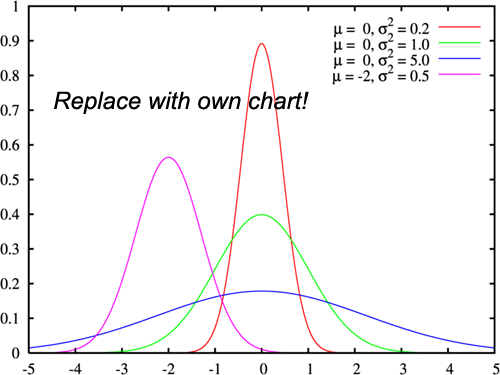
\includegraphics[width=10cm]{images/normal_distr_pdf}	
	\label{fig:gaussian_distr_pdf}
	\caption{The Normal distribution PDF.}
\end{figure}

\subsection{Equations}
By using these probabilities, and Bayes formula, we can derive the Bayes classifier.
\begin{equation}
	P(\omega_i | \boldsymbol{x}, \mathcal{X}) = \frac{p(\boldsymbol{x}|\omega_i, \mathcal(X))P(\omega_i|\mathcal{X})}{\sum_{j=1}^{c}p(\boldsymbol{x}|\omega_j, \mathcal{X})P(\omega_j|\mathcal{X})},
	\label{eq:bayes_formula_1}
\end{equation}
when we can separate the training samples by class into $c$ subsets $\mathcal{X}_1, \ldots, \mathcal{X}_c$, with the samples in $\mathcal{X}_i$ belonging to $\omega_i$.

